\section{Застосування алгоритму Бойкова-Колмогорова}

Введемо поняття \textbf{маски рухомих об'єктів}.

Маскою рухомих об'єктів кадру \(F^{i}\) будемо називати бінарне
зображення \(B^{i}:P \rightarrow \left\{ 0,1 \right\}\), де тим
пікселям, в яких на відповідному кадрі \(F^{i}\) було помічено рух,
відповідає одиниця, а іншим відповідає нуль. Для обраного користувачем
кроку \(s > 0\) на двох кадрах \(F^{i}\) і \(F^{i + s}\) рухомі об'єкти
являють собою підмножину пікселів, колір яких було змінено більше, ніж
на певне значення, з урахуванням зміни кольорів у сусідніх пікселях.
Тобто, якщо рухомий об'єкт складається з одного пікселя, його рух може
бути проігнорованим в залежності від обраних користувачем налаштувань,
про які йдеться мова далі; аналогічно, якщо рухомий об'єкт на кадрі
містить нерухомі «дірки» (пікселі, де колір не змінився), вони можуть
вважатися частиною рухомого об'єкту.

\begin{figure}[H]
	\centering
	\begin{subfigure}[b]{0.55\textwidth}
		\centering
		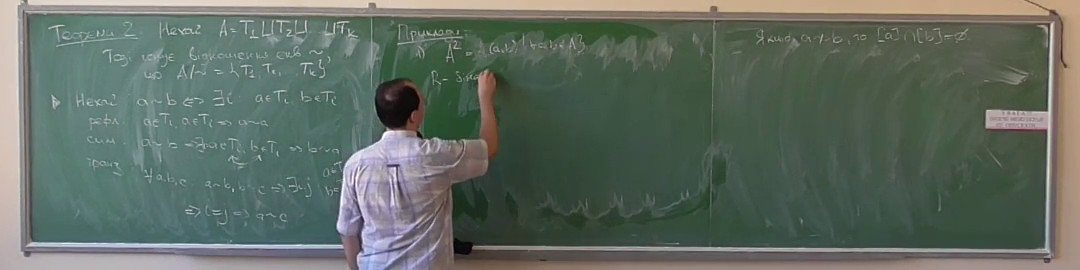
\includegraphics[width=\textwidth]{images/prev_frame}
		\caption{Попередній кадр $F^i$
			\label{fig:yakovlev:bk_examples:a}
		}
	\end{subfigure}
	
	\begin{subfigure}[b]{0.55\textwidth}
		\centering
		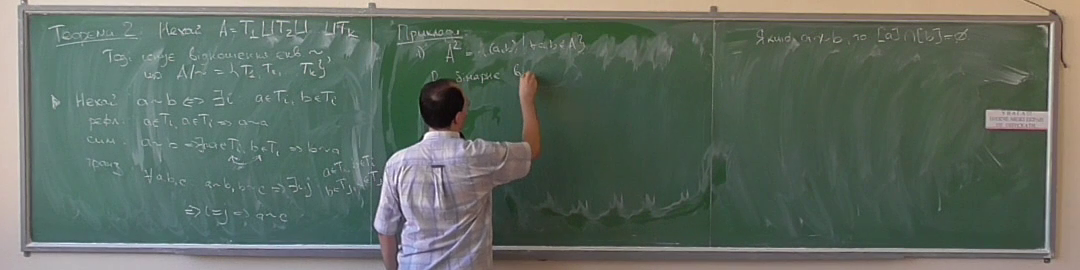
\includegraphics[width=\textwidth]{images/next_frame}
		\caption{Поточний кадр $F^{i+s}$
			\label{fig:yakovlev:bk_examples:b}
		}
	\end{subfigure}
\end{figure}
\begin{figure}[H]
	\centering
	\ContinuedFloat
	\begin{subfigure}[b]{0.55\textwidth}
		\centering
		
\includegraphics[width=\textwidth]{images/inv_diff}
		\caption{Інвертована різниця $F^i$ і $F^{i+s}$
			\label{fig:yakovlev:bk_examples:c}
		}
	\end{subfigure}
	
	\begin{subfigure}[b]{0.55\textwidth}
		\centering
		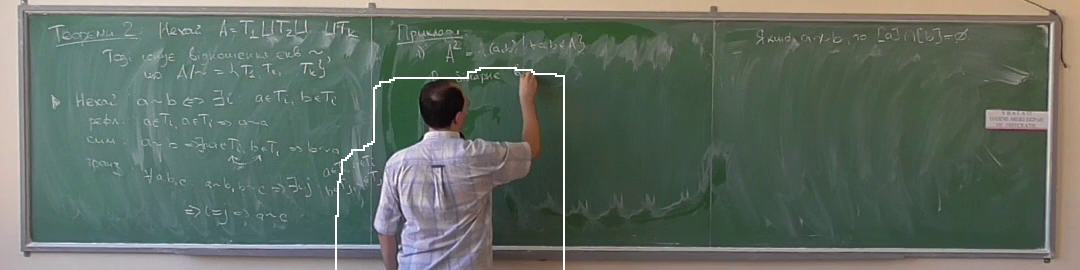
\includegraphics[width=\textwidth]{images/next_with_mask}
		\caption{Маска рухомих об'єктів на кадрі $F^{i+s}$
			\label{fig:yakovlev:bk_examples:d}
		}
	\end{subfigure}
	
	\caption{Процес створення маски рухомих об'єктів з відео \cite{yakovlev_video}
		\label{fig:yakovlev:bk_examples}
	}
\end{figure}


Для того, щоб видалити всі рухомі об'єкти, які можуть перекривати дошку, ми
беремо кадри \(F^{i}\) та \(F^{i + s}\)  ( рис. \ref{fig:yakovlev:bk_examples},
\subref{fig:yakovlev:bk_examples:a},
\subref{fig:yakovlev:bk_examples:b}) та для
кожної пари кольорів пікселів \(p\) з однаковими координатами знаходимо
модуль \(D_{p}^{i} = \left| F_{p}^{i} - F_{p}^{i + s} \right|\) різниці
інтенсивностей (Рис. 2 (в)). Зображення \(D^{i}\) подаємо на вхід
алгоритму Бойкова-Колмогорова.

Треба знайти маску $B^{i}:P \rightarrow \{0,1\}$ рухомих
об'єктів для кадрів \(F^{i}\) і \(F^{i + s}\).
Введемо функції.

\begin{equation}
	q_{p}(B_{p}^{i}) =
	\begin{gathered}
		\begin{cases}
			\alpha D_{p}^{i}, & якщо\ B_{p}^{i} = 0 \\
			255 - D_{p}^{i},  & якщо\ B_{p}^{i} = 1 
		\end{cases}
	\end{gathered}
\end{equation}

\begin{equation}
	g(B_{p}^{i},B_{p'}^{i}) = \beta|B_{p}^{i} - B_{p'}^{i}|
\end{equation}

де \(\alpha\) та \(\beta\) -- параметри згладжування маски, що задаються
користувачем інформаційної технології. Позначимо множину
$\Gamma \subset P^{2}$ сусідніх пікселів. У даній роботі сусідніми до
пікселя \(p \in P\) вважаються пікселі з множини
\(\left\{ \left( p_{x + 1},p_{y} \right),\left( p_{x},p_{y + 1} \right) \right\} \cap P\).
Сформулюємо пошук маски \(B^{i}\) у вигляді задачі мінімізації виразу

\begin{equation}
	E\left( B_{p}^{i} \right) = \sum_{p \in P}^{}{q_{{p\ }}( B_{p}^{i}) +}\sum_{(p,p') \in \Gamma}^{}g(B_{p}^{i},B_{p'}^{i})
\end{equation}


На виході отримуємо маску \(B_{p}^{i}\) рухомих об'єктів ( рис.
\ref{fig:yakovlev:bk_examples:d} ).
Її ми використовуємо, щоб не переносити на фінальне зображення ті
пікселі, на яких було помічено рух, адже зміна яскравості пікселя
виникає не тільки під час створення напису, а й під час тимчасового
затуляння дошки.

% \textbf{Переваги методу:}
% \begin{enumerate}
% 	\item Алгоритм Б-К досить швидко будує мінімальний розріз. Статистика на ОС
% 	      Ubuntu 21.04 під Intel Core i5-7200U @ 4x 3,1GHz, час 0.15 секунди на
% 	      кадрі розмірами 330х640.
% 	\item Даний метод не потребує ніякої передобробки, тобто не потрібно навчати
% 	      як нейронну мережу.
% \end{enumerate}

% \textbf{Недоліки методу:}
% \begin{enumerate}
% 	\item Оскільки даний метод локалізує рух на кадрах відео, то коли
% 	      рухається камера, відповідно практично все що в кадрі стає рухомим об'єктом (рис.
% 	      \ref{fig:seminar:bad_example}). Це може давати дефекти на панорамних знімках. В
% 	      розділі № описано як була поборена дана проблема.
% 	      % Межкафедральный семинар (семинар), Райгородский А. М., 29.03.2022г.
% 	      \begin{figure}[H]
% 	      	\centering
% 	      	\begin{subfigure}[c]{0.4\textwidth}
% 	      		\centering
% 	      		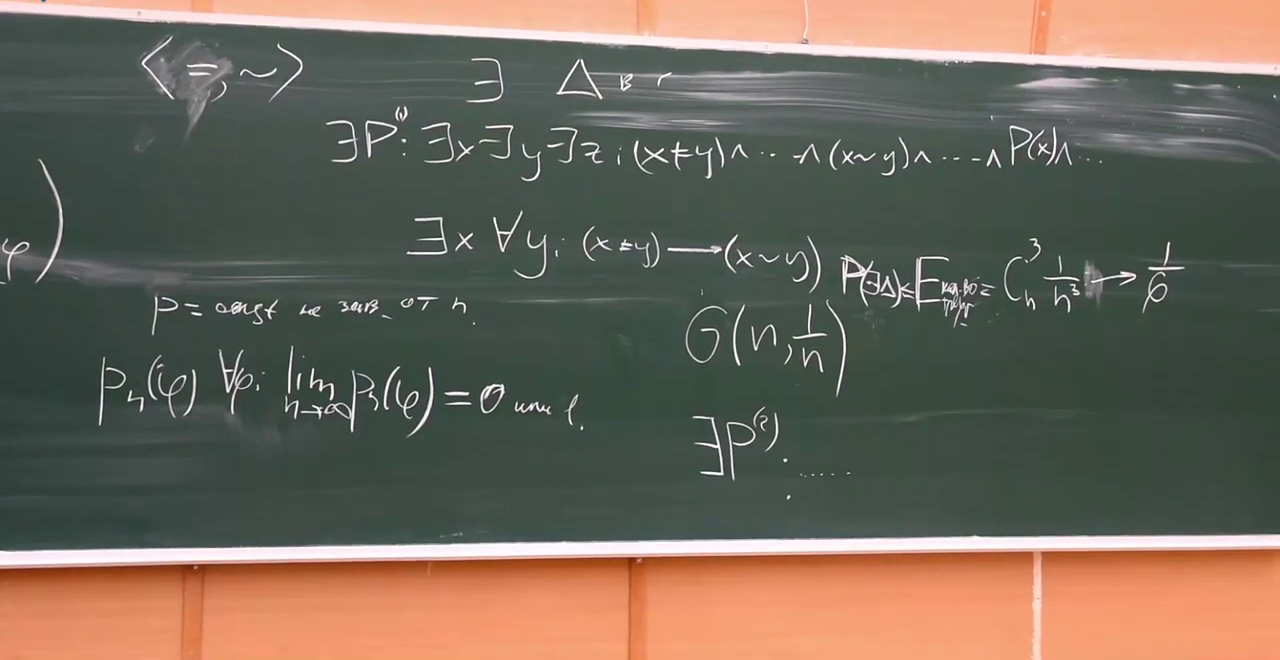
\includegraphics[width=\textwidth]{images/bad_example_1}
% 	      		\caption{Попередній кадр
% 	      			\label{fig:seminar:bad_example:a}
% 	      		}
% 	      	\end{subfigure}
% 	      	\begin{subfigure}[c]{0.4\textwidth}
% 	      		\centering
% 	      		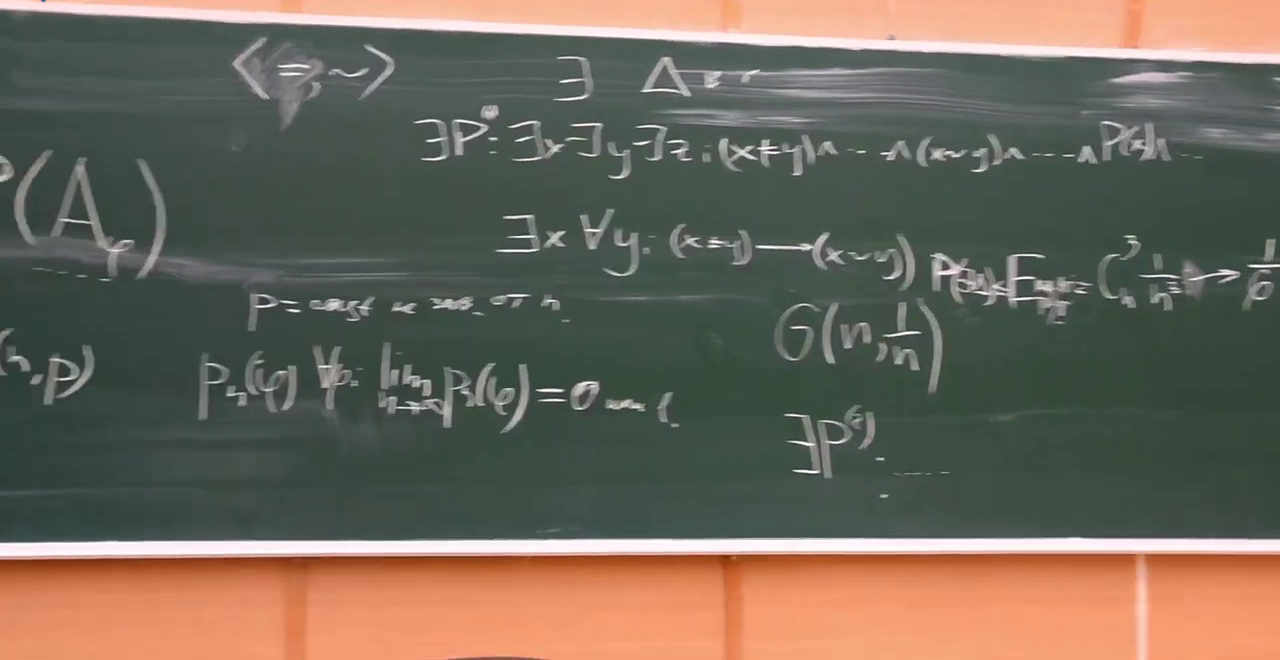
\includegraphics[width=\textwidth]{images/bad_example_2}
% 	      		\caption{Поточний кадр
% 	      			\label{fig:seminar:bad_example:b}
% 	      		}
% 	      	\end{subfigure}
% 	      \end{figure}
% 	      \begin{figure}[H]
% 	      	\centering
% 	      	\ContinuedFloat
% 	      	\begin{subfigure}[c]{0.4\textwidth}
% 	      		\centering
% 	      		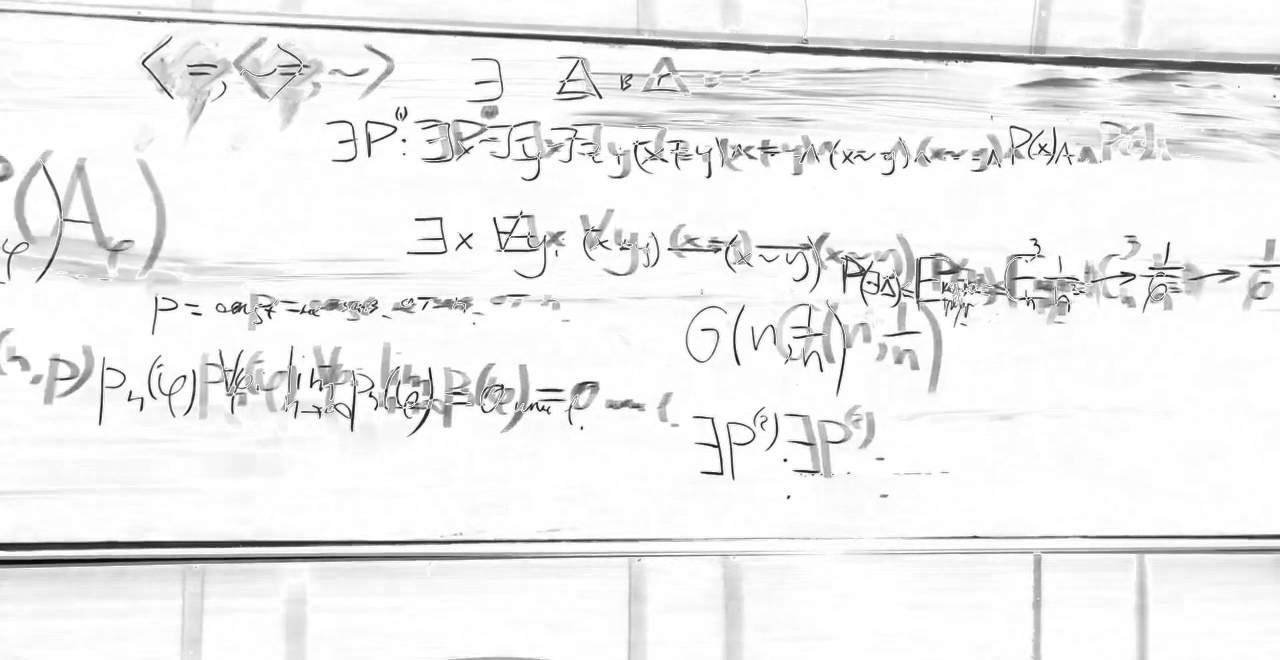
\includegraphics[width=\textwidth]{images/bad_example_inv_dif}
% 	      		\caption{Інвертована різниця
% 	      			\label{fig:seminar:bad_example_inv:c}
% 	      		}
% 	      	\end{subfigure}
% 	      	\begin{subfigure}[c]{0.4\textwidth}
% 	      		\centering
% 	      		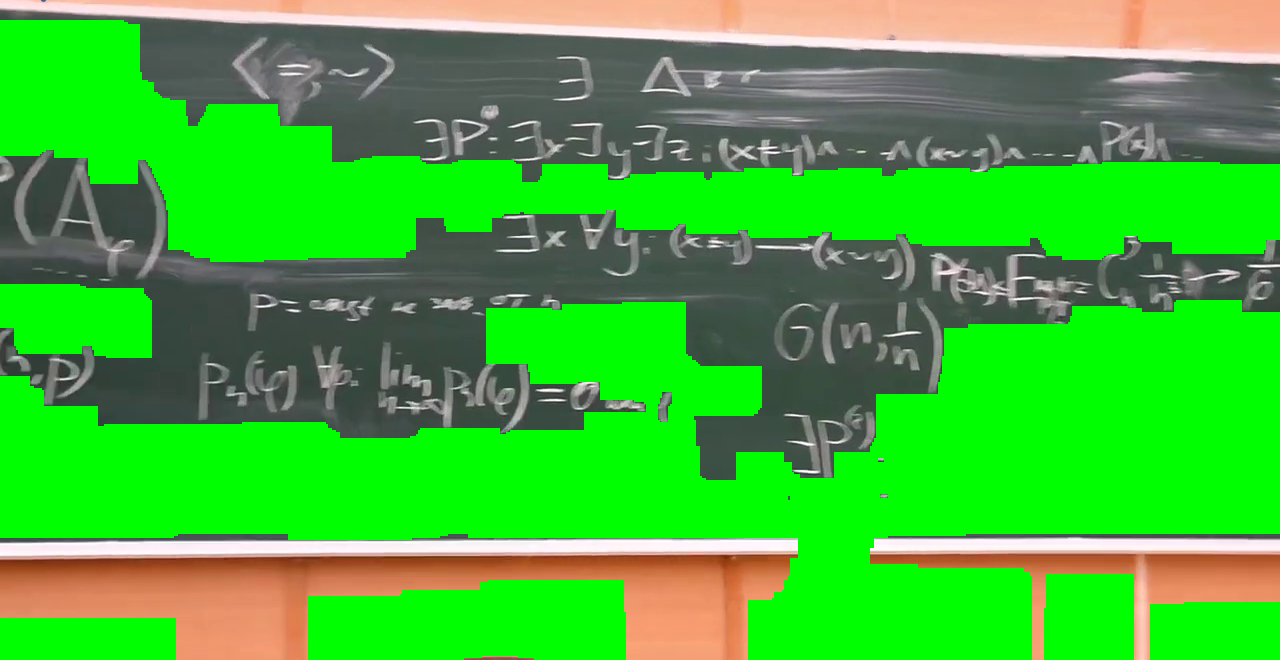
\includegraphics[width=\textwidth]{images/bad_example_mask}
% 	      		\caption{Маска рухомих об'єктів
% 	      			\label{fig:seminar:bad_example_mask:c}
% 	      		}
% 	      	\end{subfigure}
	      	
% 	      	\caption{Приклад отримання поганої маски під час руху камери
% 	      		\label{fig:seminar:bad_example}
% 	      	}
% 	      \end{figure}
	      
% 	\item Якщо викладач практично не рухається довгий час, відповідно не потрапляє
% 	      на маску рухомих об'єктів, то він може потрапити на
% 	      панорамний знімок.
% \end{enumerate}
